Since \drunkened\ is a public display game, it has to have several properties:
\begin{itemize}\compresslist
\item It must be very easy to understand and to play. Therefore, the game is reduced to one main input (the upper body) and one simple goal (walking to the right).
\item One game session must be quite short. The game and also public display games in general are targeting people, which are actually not planning to play. Therefore, they might not want to spent to much time with a game, that they started spontaneously. Furthermore, \drunkened\ is a single player game, so players have to take turns, which is easier with short game sessions.
\marginpar{
\begin{figure}
  \centering
  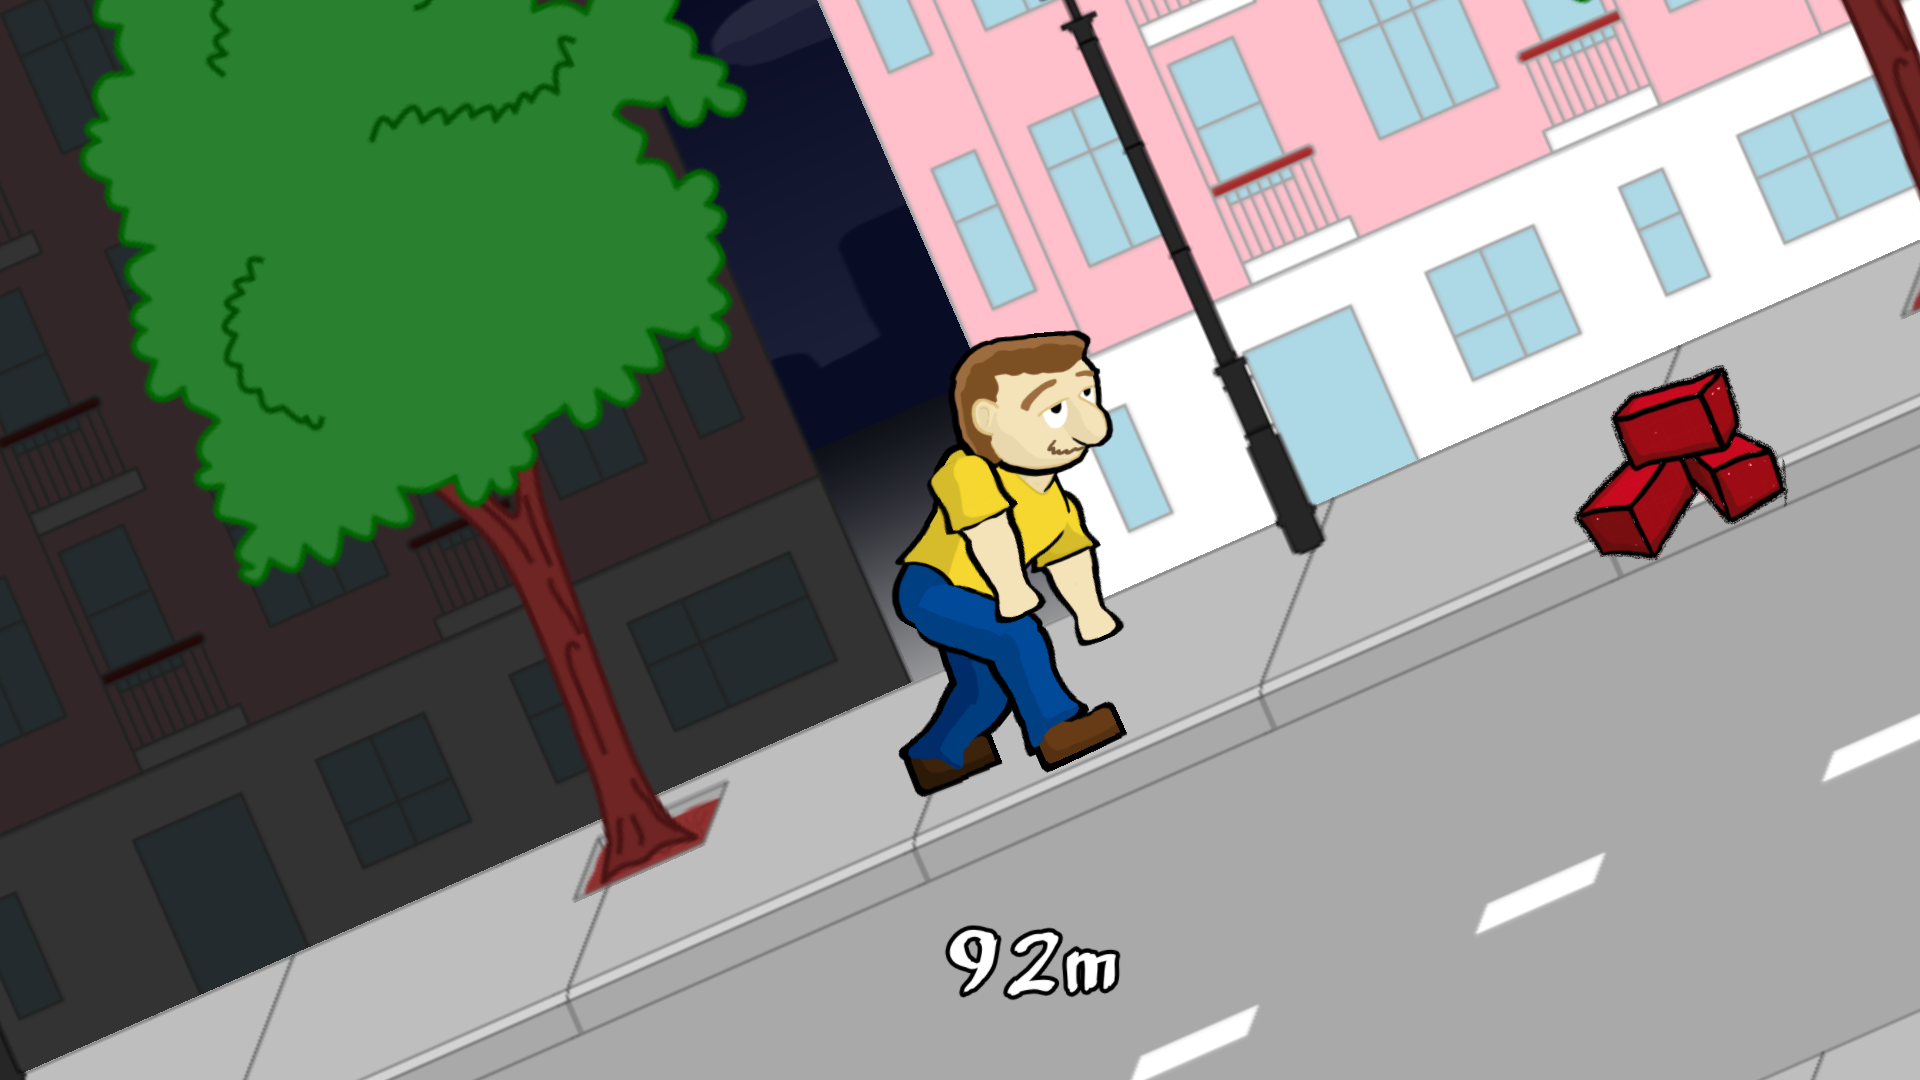
\includegraphics[width=\linewidth]{pictures/screenshot1.png}
  \caption{Insert a caption below each figure.}
  \label{fig:screenshot1}
\end{figure}
\begin{figure}
  \centering
  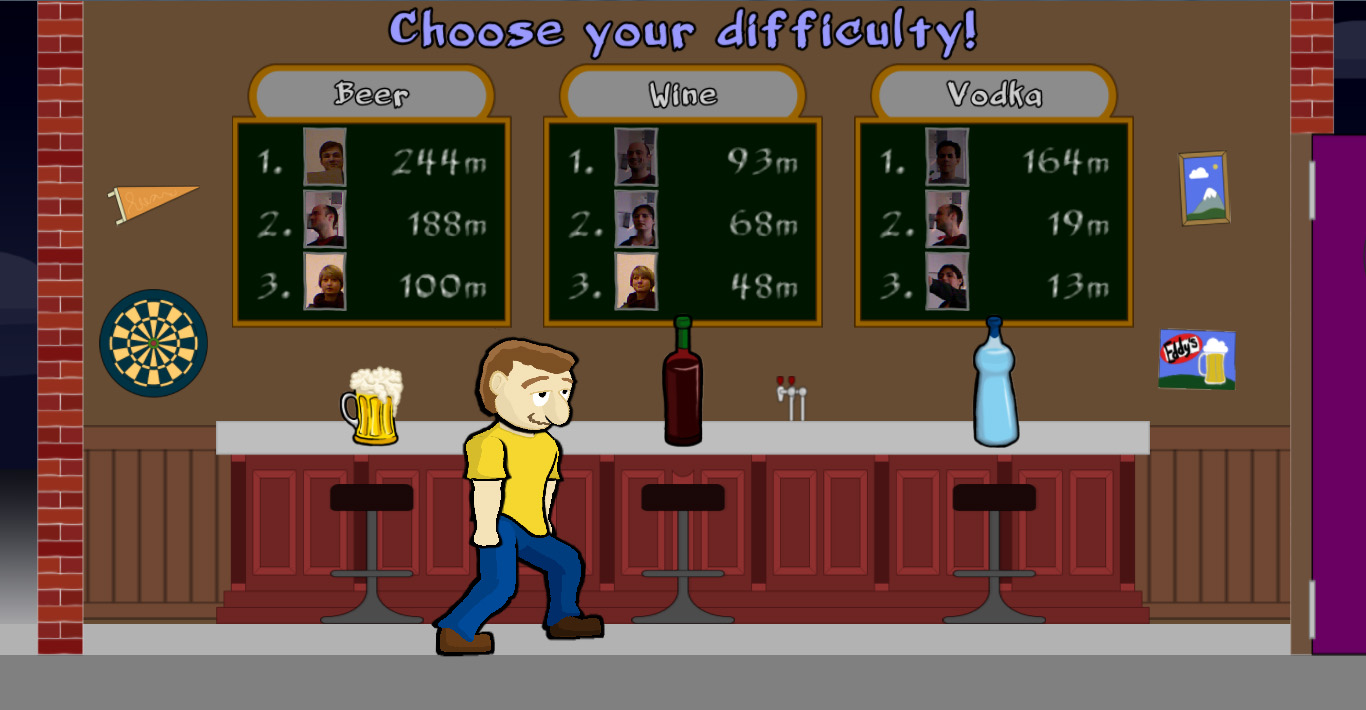
\includegraphics[width=\linewidth]{pictures/screenshot2.jpg}
  \caption{Insert a caption below each figure.}
  \label{fig:screenshot2}
\end{figure}
\begin{figure}
  \centering
  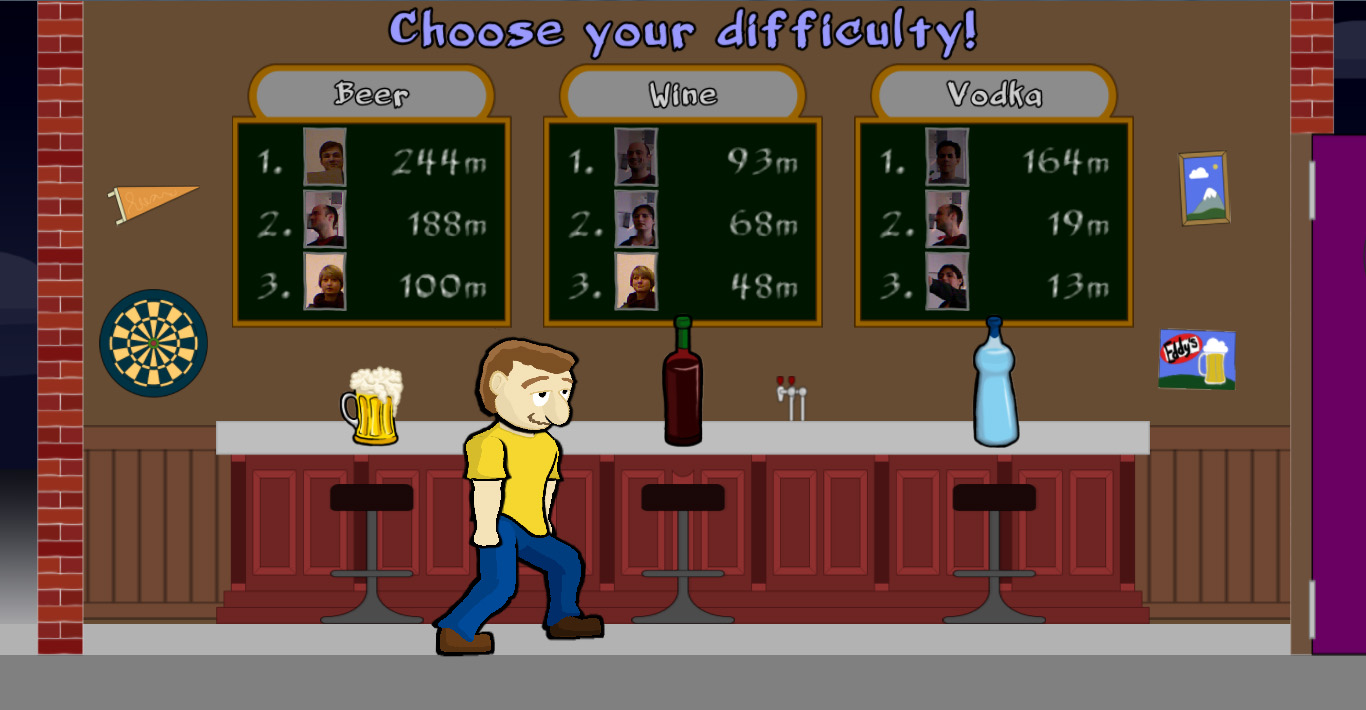
\includegraphics[width=\linewidth]{pictures/screenshot2.jpg}
  \caption{Insert a caption below each figure.}
  \label{fig:screenshot3}
\end{figure}
\begin{figure}
  \centering
  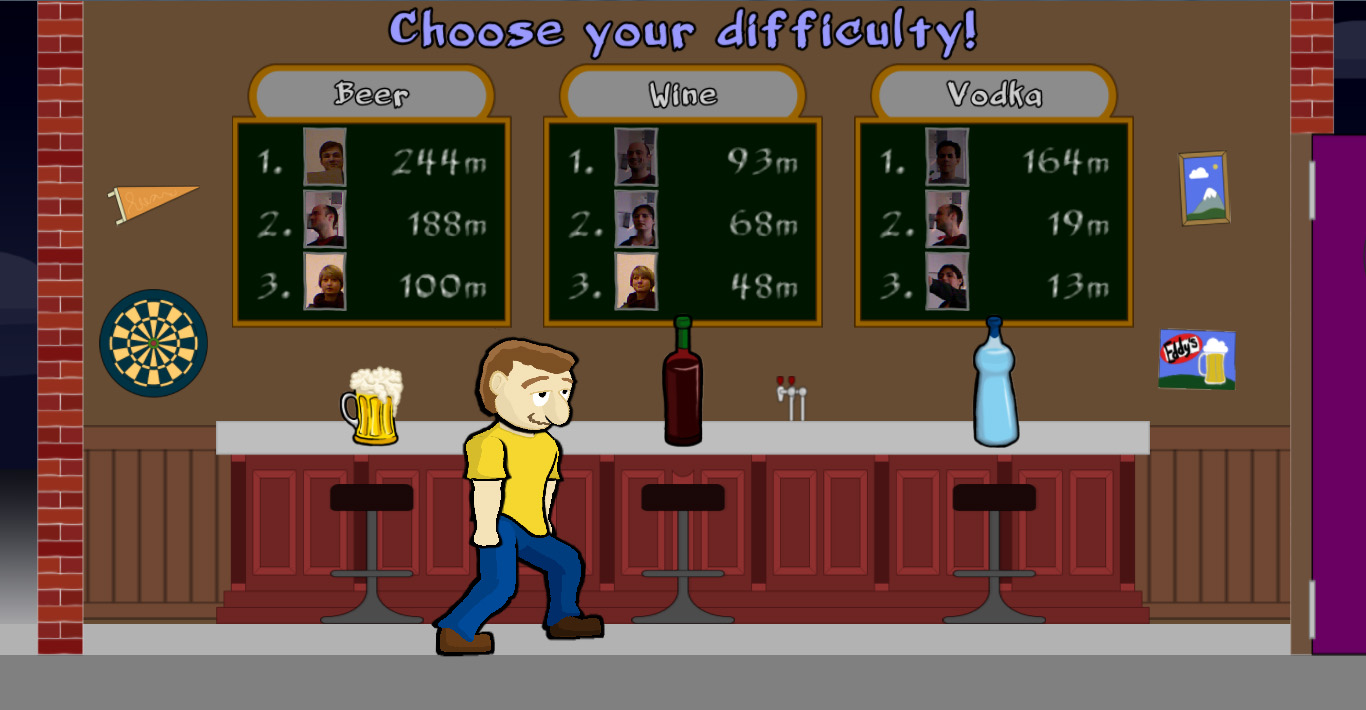
\includegraphics[width=\linewidth]{pictures/screenshot2.jpg}
  \caption{Insert a caption below each figure.}
  \label{fig:screenshot4}
\end{figure}
}
\item The narrative elements must be reduced to a minimum. There are no cutscenes, long texts etc. to tell the game's background. The animations, the players actions and keywords like ''distance'' give the game a humorous context.
\end{itemize}

\drunkened\ targets a joy of failing, that is, letting \ed\ eventually tumble and fall asleep. \eds\ tumbling is not implemented as an animation, but physics based, i.e. depending on \eds\ locomotion and angular velocity. This means, that failing varies from player to player, since they can take \ed\ into individual, often awkward, sleeping postures. This also attempts to compensate the fact, that \drunkened\ is a single player game, because spectators can have fun seeing others fail.